\chapter{Remarks about our study}
In this chapter describe in detail the specifications of the simulations we are going to work with. Furthermore, we present the chosen method for determining the halo shapes. This chapter is mainly to thoroughly explain how are we going to do everything that we are going to do.\\

\section{The Auriga simulations}
In this monograph we use the results of the state-of-the art Auriga simulations \cite{Auriga}. It selected a set of 30 isolated halos from the Eagle simulations \cite{Eagle}. Each halo was identified with a modified version of the algorithm "Friend of Friends" (FOF) \cite{FOF}, that recursively links particles if they are closer than some distanse threshold called linking length. Eagle follows the evolution of fixed-mass particles of $m_{\text{DM}} = 1.15\cdot 10^7\text{M}_{\odot}$ from $z=127$ to $z=0$. Eagle simulations adopt the cosmological model from Planck Collaboration et al. (2014) by taking the parameters $\Omega_\Lambda=0.693$, $\Omega_\text{m}=0.307$, $\Omega_\text{b}=0.048$ \& $\text{H}_0=67.77\text{kms} ^{-1}\text{Mpc}^{-1}$.\\

These halos were randomly selected from a sample of the quartile of most isolated halos whose virial mass $M_{200}$ varied between $10^{12}M_\odot$ and $2\cdot 10^{12}M_\odot$. This mass is defined as the mass enclosed within the virial radius $R_{200}$ at which the density becomes 200 times the critical density of the universe. These halos were then re-simulated by increasing the mass resolution of the particles belonging to each halo and diminishing the resolution of the rest of the particles. This would efficiently simulate external gravitational effects over the studied structure and reproduce a high-resoluted version of it.\\

Various versions of the same halo were simulated for different degrees of realism. All 30 halos were simulated within a level 4 degree of resolution defined for Aquarius simulations which corresponds to $\tilde 3\cdot 10^6$ high resolution particles of $\tilde 2.5 \cdot 10^5 M_\odot$. The principal details of each of these halos are consigned on the table \ref{tab:level4}. From these halos, 6 of them where re-simulated at level 3 (higher) resolution taking into account a spatial factor of 2 in each dimension. For more information about level 3 halos, their information is printed on table \ref{tab:level3}. Furthermore, fore each halo in each level of resolution there are two versions of the simulation. One evolves only DM particles and the other has into account all the magneto-hydrodynamical physics, including DM. Taking this into account, we can compare the results from different levels of realism to obtain consistency in our analysis.\\

\begin{table}[h!]
\centering
\begin{tabular}{l?cc?cc?cc?cc}
\hline
\hline
Halo & \multicolumn{2}{c?}{$N_P$/$10^6$} & \multicolumn{2}{c?}{$M_P$/$10^5M_\odot$} & \multicolumn{2}{c?}{$R_{vir}$/Kpc}&\multicolumn{2}{c}{$M_{vir}$/$10^{14}M_\odot$}  \\ \hdashline
& DM & MHD& DM & MHD& DM & MHD& DM & MHD\\ \hline \hline
halo 1&4.068&2.447&2.397&2.022&196.927&187.674&9.062&7.844\\
halo 2&5.625&5.457&2.481&2.093&235.094&233.934&15.418&15.191\\
halo 3&3.826&3.852&2.645&2.231&210.693&210.955&11.099&11.141\\
halo 4&4.585&4.530&2.590&2.185&219.378&215.438&12.529&11.866\\
halo 5&3.262&3.290&2.533&2.137&196.984&197.246&9.071&9.106\\ \hdashline
\rowcolor{blue!30} halo 6&3.184&3.110&2.337&1.972&191.840&189.342&8.378&8.054\\ \hdashline
halo 7&3.878&3.729&2.296&1.937&197.864&196.509&9.193&9.005\\
halo 8&2.772&2.796&2.451&2.068&190.716&191.764&8.231&8.368\\
halo 9&3.038&3.010&2.738&2.310&195.826&190.640&8.911&8.222\\
halo 10&2.700&2.751&2.541&2.144&187.139&188.147&7.777&7.904\\
halo 11&4.146&4.116&2.541&2.144&221.821&219.568&12.952&12.560\\
halo 12&2.865&2.908&2.645&2.231&192.280&192.038&8.436&8.404\\
halo 13&3.520&3.600&2.393&2.019&202.139&203.815&9.801&10.048\\
halo 14&4.200&4.475&2.499&2.108&215.535&218.927&11.882&12.453\\
halo 15&2.888&2.845&2.541&2.144&199.848&200.658&9.471&9.588\\ \hdashline
\rowcolor{blue!30} halo 16&3.821&3.871&2.499&2.108&212.590&212.632&11.401&11.408\\ \hdashline
halo 17&2.752&2.781&2.552&2.153&188.067&187.404&7.893&7.811\\
halo 18&3.770&3.624&2.738&2.310&201.124&207.293&9.655&10.571\\
halo 19&2.989&3.086&2.645&2.231&200.244&200.325&9.527&9.540\\
halo 20&3.903&3.822&2.481&2.093&210.097&211.423&11.005&11.214\\ \hdashline
\rowcolor{blue!30} halo 21&4.105&4.075&2.640&2.227&219.527&219.823&12.555&12.604\\ \hdashline
halo 22&2.794&2.766&2.625&2.215&188.363&184.801&7.931&7.489\\ \hdashline
\rowcolor{blue!30} halo 23&3.977&4.073&2.795&2.358&217.768&215.959&12.254&11.952\\\hdashline
\rowcolor{blue!30} halo 24&4.466&4.426&2.522&2.127&217.440&215.147&12.199&11.817\\ \hdashline
halo 25&2.902&2.806&2.645&2.231&199.922&198.299&9.482&9.254\\
halo 26&4.610&4.716&2.506&2.115&219.984&218.939&12.633&12.454\\\hdashline
\rowcolor{blue!30} halo 27&5.060&5.018&2.590&2.185&228.036&226.225&14.071&13.740\\ \hdashline
halo 28&4.184&4.276&2.645&2.231&216.979&217.997&12.121&12.294\\
halo 29&4.827&4.613&2.499&2.108&225.791&219.935&13.660&12.625\\
halo 30&3.268&3.112&2.579&2.176&195.043&194.741&8.805&8.763\\
\hline
\hline
\end{tabular}
\caption{Specifications of each level 4 galaxy (halo). The DM and MHD versions of each parameters are presented together. The columns of this table indicate: (1) Halo name, (2,3) Number of (millions) of DM particles belonging to the halo, (4,5) Mass per particle in $10^5M_\odot$, (6,7) Virial radius (R TopHat 200) of the halo in Kpc, (8,9) Virial mass of the halo in $10^{14}M_\odot$.}
\label{tab:level4}
\end{table} 

\begin{table}[h!]
\centering
\begin{tabular}{l?cc?cc?cc?cc}
\hline
\hline
Halo & \multicolumn{2}{c?}{$N_P$/$10^6$} & \multicolumn{2}{c?}{$M_P$/$10^5M_\odot$} & \multicolumn{2}{c?}{$R_{vir}$/Kpc}&\multicolumn{2}{c}{$M_{vir}$/$10^{14}M_\odot$}  \\ \hdashline
& DM & MHD& DM & MHD& DM & MHD& DM & MHD\\ \hline \hline
halo 6&24.902&24.185&0.292&0.246&191.741&188.367&8.365&7.932\\
halo 16&29.750&30.334&0.312&0.263&212.622&212.542&11.406&11.395\\
halo 21&31.993&31.503&0.330&0.278&219.731&220.250&12.588&12.679\\
halo 23&31.379&31.618&0.349&0.295&217.793&213.358&12.259&11.524\\
halo 24&34.987&35.153&0.315&0.266&217.313&213.963&12.179&11.624\\
halo 27&39.617&39.056&0.324&0.273&227.908&223.484&14.048&13.244\\
\hline
\hline
\end{tabular}
\caption{Specifications of each level 3 galaxy (halo). The DM and MHD versions of each parameters are presented together. The columns of this table indicate: (1) Halo name, (2,3) Number of (millions) of DM particles belonging to the halo, (4,5) Mass per particle in $10^5M_\odot$, (6,7) Virial radius (R TopHat 200) of the halo in Kpc, (8,9) Virial mass of the halo in $10^{14}M_\odot$.}
\label{tab:level3}
\end{table} 

\begin{figure}[!ht]
    \centering
    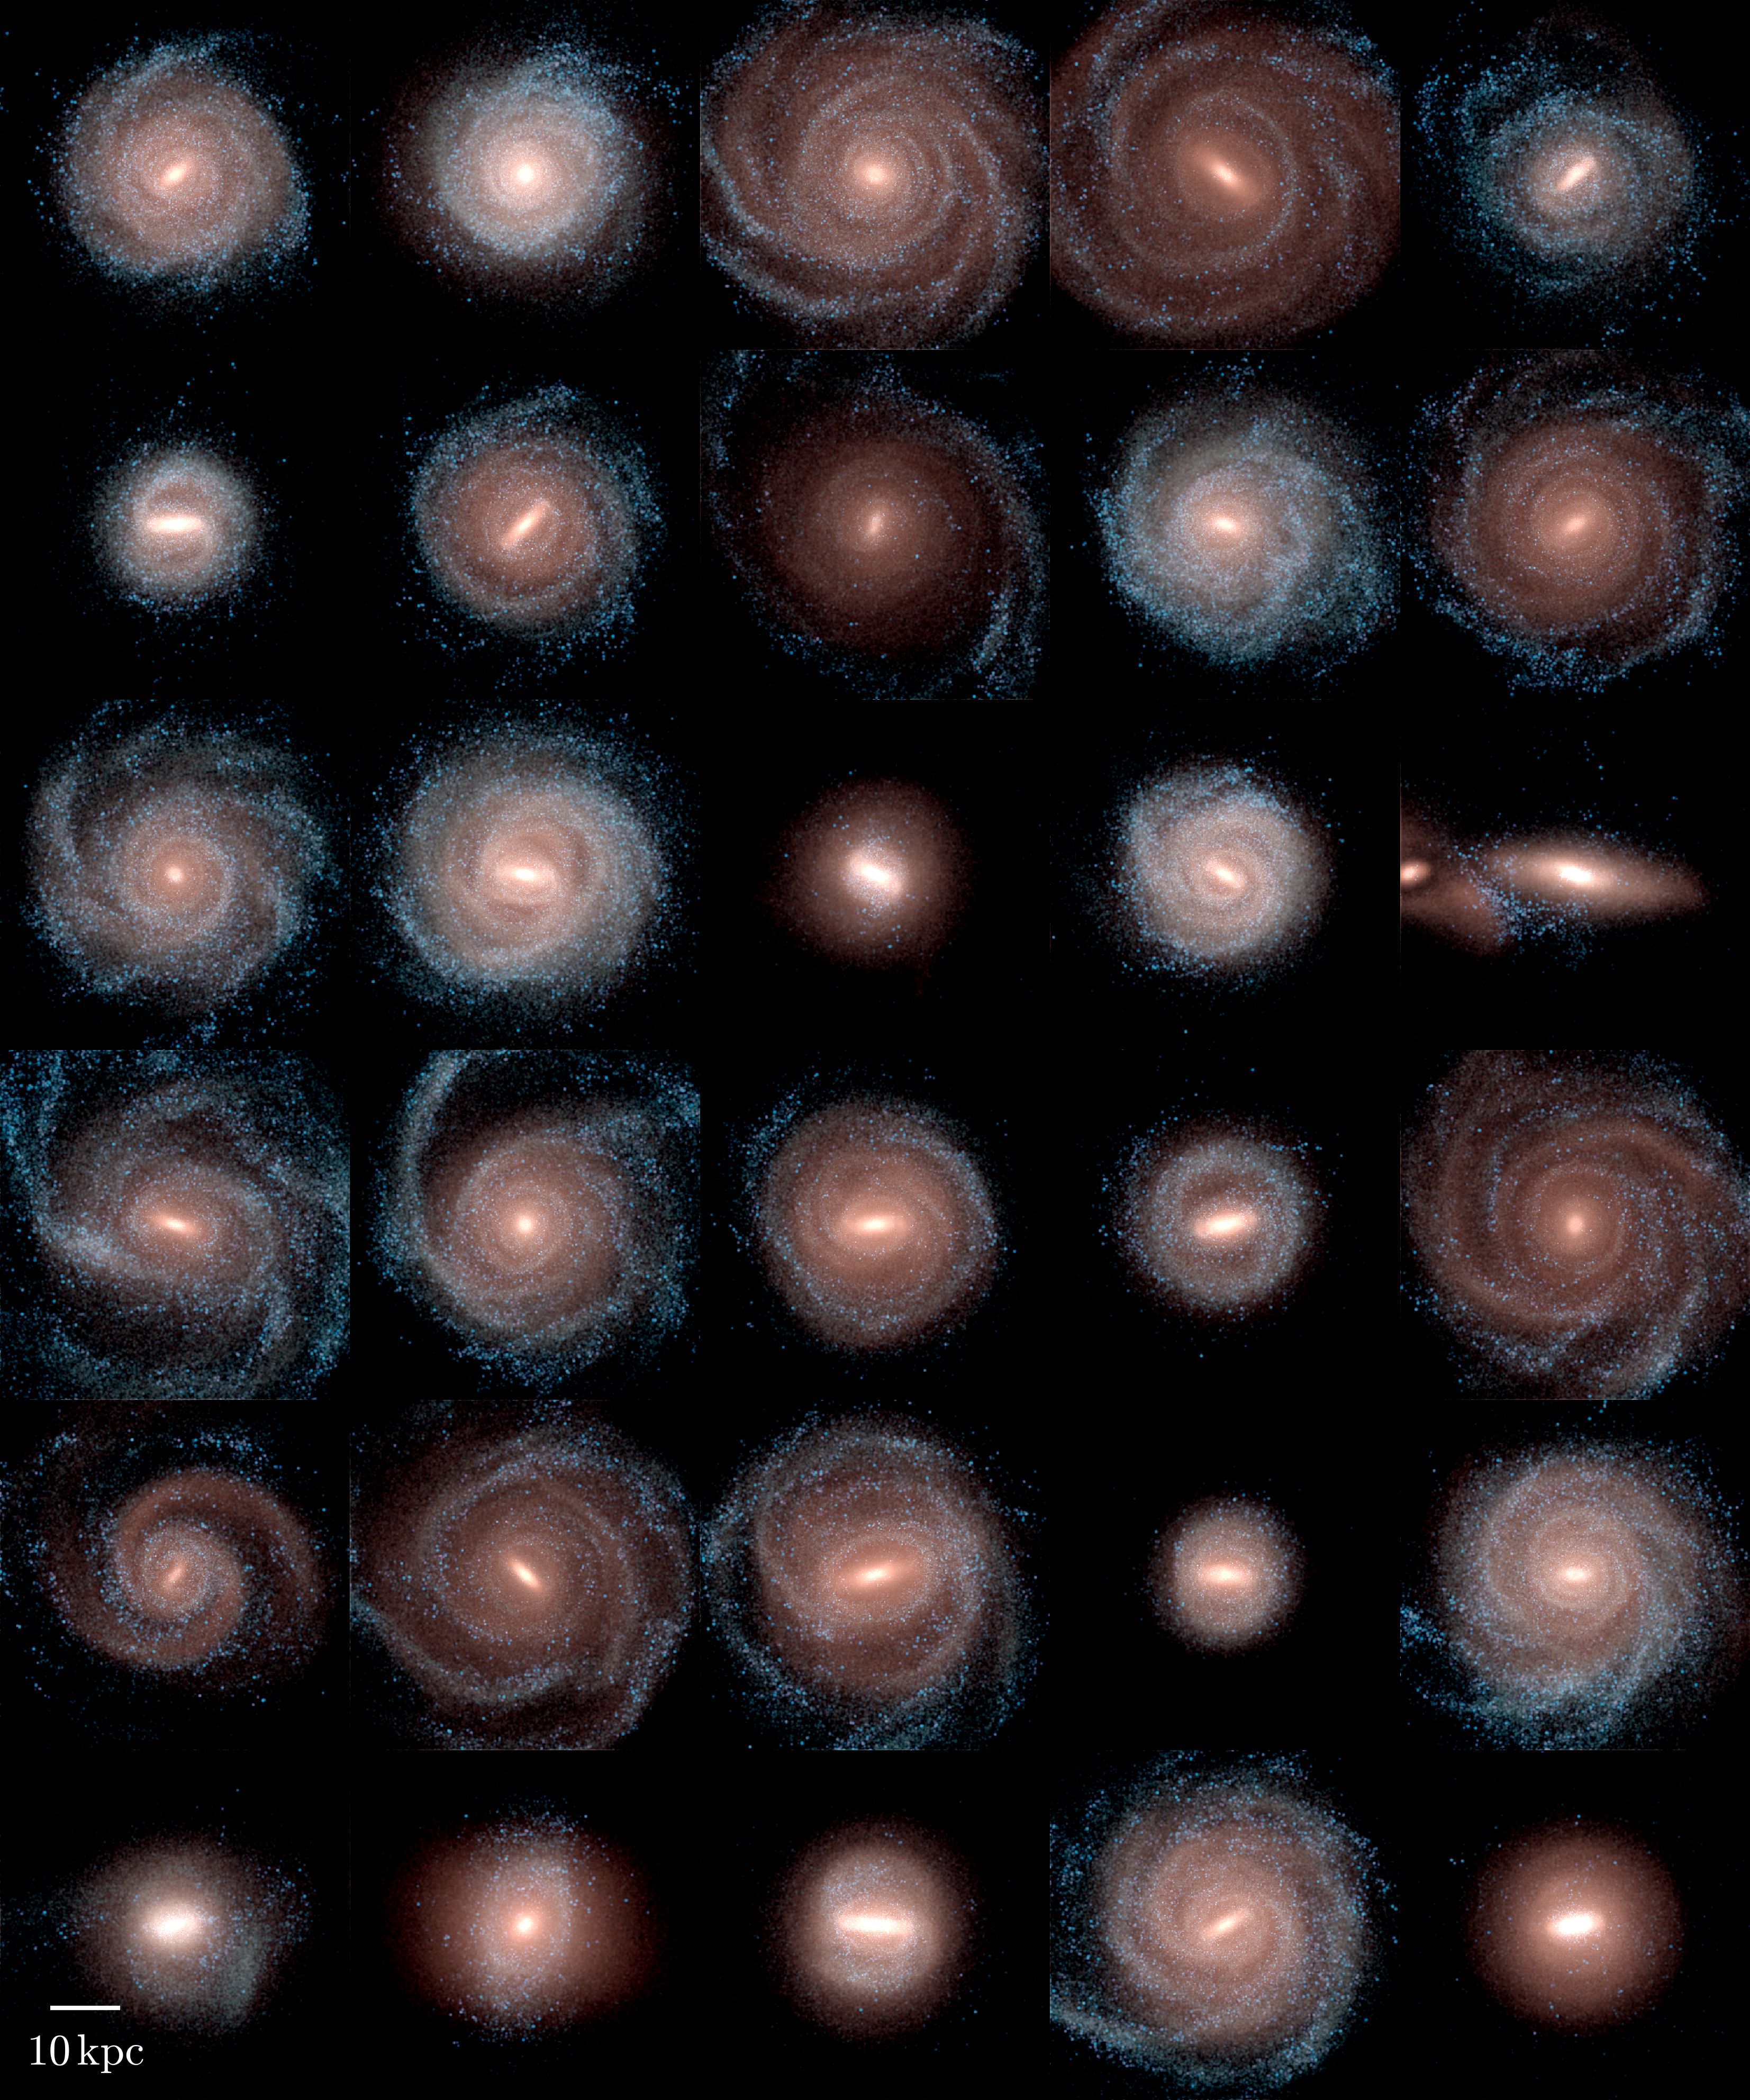
\includegraphics[width=0.8\textwidth]{./pics/Auriga.png}
    \caption{Set of 30 MW-like simulations from Auriga, taken from http://auriga.h-its.org/}
    \label{fig:auriga}
\end{figure}


\section{Determining the halo shape}
The discretization of the DM density field into particles makes it difficult  to perform some calculations that would require a more continuous distribution such as those related to the density field. The case of the shape of the halo is no exemption, and therefore there is no trivial way to calculate the DM halo shape at a determined radius. There are different approaches to this problem, such as the use of an inertia tensor or the approximation to the respective contour surface.
However, the results do not vary very much from method to method \cite{Vera-Ciro et al. 2011}. In this work we follow the guidelines by Vera-Ciro et al 2011 which includes the use of the shape method by Allgood 2006\cite{AllGood2006}.\\

Allgood's method starts with particles enclosed within a sphere whose radius $r$ is the initial radius where we want to obtain the shape. We calculate the reduced inertia tensor:

\begin{equation}
I_{ij} = \sum_k \frac{x_k^{(i)}x_k^{(j)}}{d^2_k},
\label{eq:inertia}
\end{equation}

which has weighted components by distance $d^2=x^2+y^2+z^2$, so that each particle contribute with same importance to the inertia tensor, neglecting their distance to the center of the halo.\\

The diagonalization of this tensor yields the principal axes of the structure, as well as the eigen-quantities $a>b>c$ which produce the respective axial ratios. However, if we characterize an ellipsoid taking into account only particles enclosed within a sphere, we are effectively underestimating its triaxiality \cite{AllGood}. For this reason, we iteratively recalculate the inertia tensor taking into account the previously characterized ellipsoid.\\

AllGood et al. propose to use the eigenvalues $a>b>c$ and their respective eigen-axes $v_a,v_b,v_c$ to recalculate the inertia tensor over the particles enclosed by the ellipsoid with principal axes (along the respective eigenvectors) equal to $r,r/q,r/s$, where ere $q = b/a$ and $s=c/a$ are the axial ratios. In other words, we repeat the process of calculating the inertia matrix by taking into account particles within an ellipsoid with axial ratios given by the previous diagonalization, maintaining the principal axis of the enclosing ellipsoid constant (this is a freedom choice).\\

This method sounds good and it would eventually converge to a more accurate characterization of the halo ellipsoid. However, we are computing the reduced inertia tensor by weighting the contributions with the spherical-metric distance $d^2=x^2+y^2+z^2$, where particles within the same spherical surface are given the same importance. This means we are again underestimating ??? the triaxiality of the structure. For this reason, on each iteration we must calculate the inertia tensor taking into account an elliptic metric: $\bar{d}^2 = x^2+y^2/q^2+z^2/s^2$, assuming $x,y,z$ are the corresponding principal axes.\\

In case this concept of an elliptic metric is difficult to grasp, let us consider that, instead of converting the initial enclosing sphere to the halo ellipse, we are converting the halo ellipsoid into an sphere by performing scale transforms along the respective eigen-axes. From this point of view, we start our first-guess calculation of the ellipsoid by calculating the reduced inertia tensor \eqref{eq:inertia} for particles enclosed within a sphere of radius $r$. Then with the results of this first guess, we perform the following scale transform:\\
  
\begin{align}
(x,y,z) &\rightarrow (x',y',z')=(x,y/q,z/s) \label{eq:scale}\\
q &=  b/a \nonumber \\
s &= c/a \nonumber ,
\end{align}

where we assumed the axes $x,y,z$ are oriented at the principal axes. We then repeat the process of calculating the reduced inertia tensor and performing the scale transform until we achieve certain convergence criterion. We stop this iterative process when the sum of the fractional change in axes is less than $10^{-6}$ to obtain the shape of the halo at the geometric mean radius $(abc)^{1/3}$, which is not much different from the initial radius.\\

Notice that calculating the inertia tensor with the scaled coordinates $x',y',z'$ is equivalent to calculating it with the un-scaled coordinates $x,y,z$ but using the elliptic-metric distance $\bar{d}^2 = x^2+y^2/q^2+z^2/s^2$, for diagonalization purposes.\\

